	\large \bf{\textsc{\section{Lab 2}}
	\begin{problem}
		In this exercise, we would like to build a thermometer using an NTC sensor. The NTC sensor is a resistance that decreases when the temperature increases. Choose an NTC sensor with nominal value of 10K\(\Omega\) (usually given at 25$^\circ$C.
		\newline
		1. Measure the resistance of the NTC using a multimeter at the room temperature (don't touch the sensor when measuring). Let's assume that the room temperature is about 22$^\circ$C.
		\newline
		2. Measure the resistance of the NTC using a multimeter while you keep the sensor in your hands for about 30 seconds. Let's assume that your hands has the temperature of about 35$^\circ$C.
		\newline
		3. Build the following circuit with: \\
		R\(_{1}\): 10K\(\Omega\)(NTC sensor), R\(_{2}\): 10K\(\Omega\), R\(_{3}\): 4.7K\(\Omega\), R\(_{4}\): 1.8K\(\Omega\), V: 1.45V
		\newline
		4. Calculate the voltage of V\(_{OC}\) for two cases (room temperature and the hand temperature).
		\newline
		5. Measure the voltage of V\(_{OC}\) for two cases and compare the results with your calculations.
		\iffalse
		\begin{figure}[h!]
			\centering
			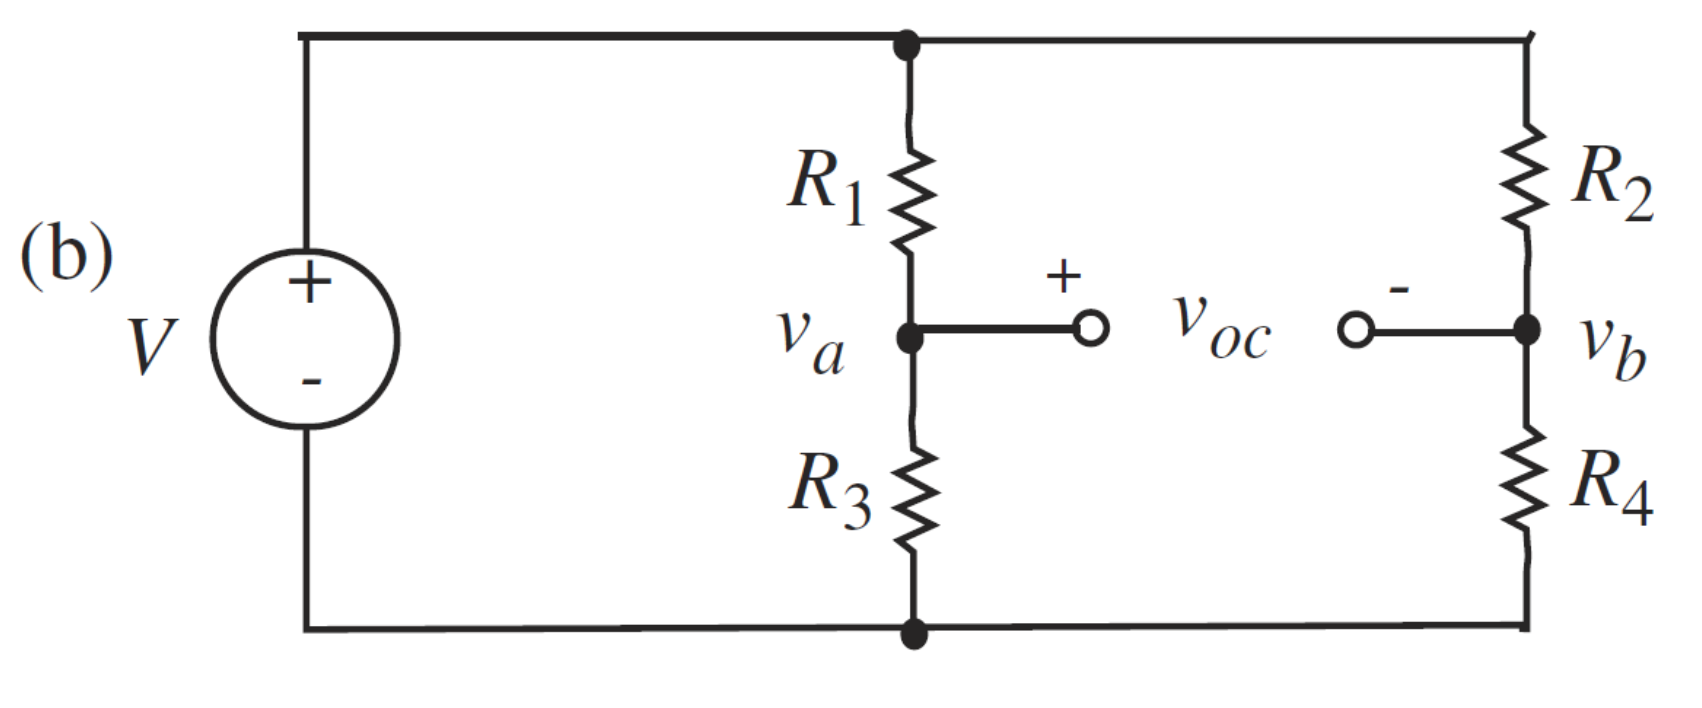
\includegraphics[width=0.5\textwidth]{images/circuit7.png}
		\end{figure}
		\fi
	\end{problem}
	
	\begin{solution}
		1. The resistance of the NTC is 10.98 k \(\Omega\) with the room temperature at about 22$^\circ$C.
		\newline
		2. The resistance of the NTC is 7.22 k \(\Omega\) when held by hand at about 35$^\circ$C.
		\newline
		3. We did the circuit in the Electrical lab.
		\newline
		4. To calculate the V$_{OC}$ we need to simplify the circuit using Thevenin Theorem. In the first case, we look at room temperature, where R$_{1}=10.98$k\(\Omega\).
		
		$R_{13}=(10.98*4.7)/(10.98+4.7)\approx3.29k\Omega$
		
		$R_{24}=(10*1.8)/(10+1.8)\approx1.52k\Omega$
		
		\begin{figure}[h!]
			\centering
			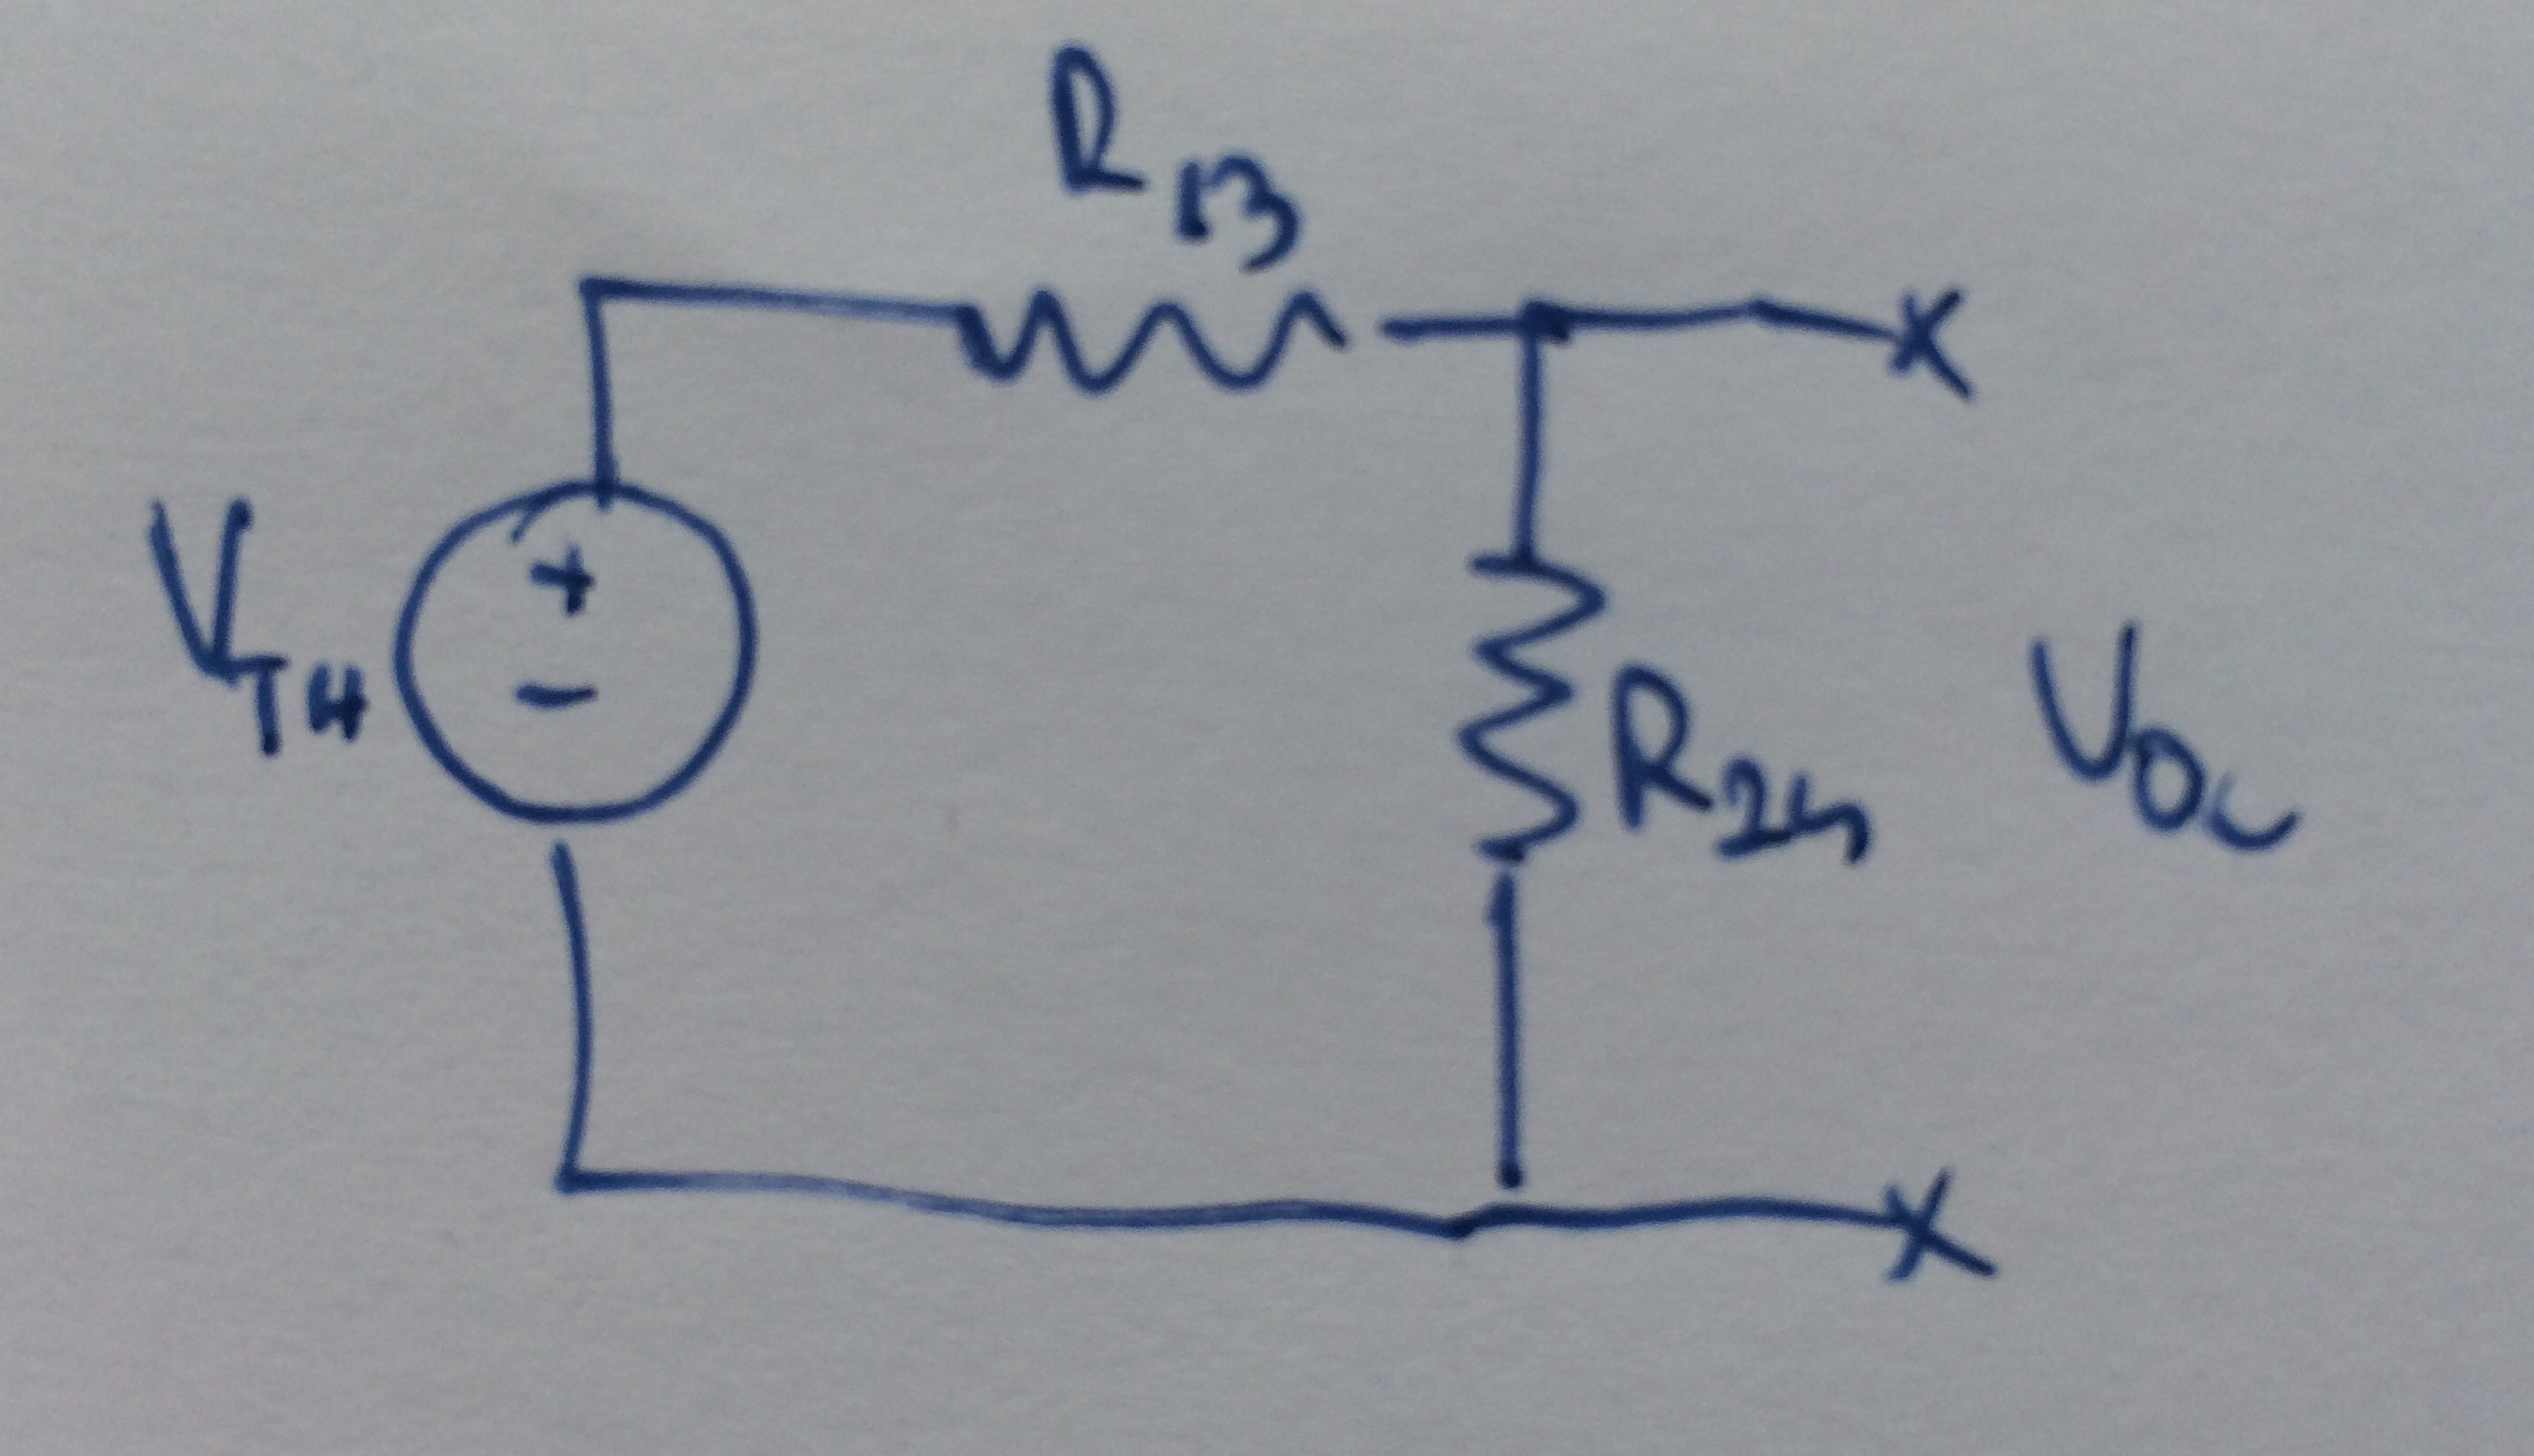
\includegraphics[width=0.3\textwidth]{images/circuit214.jpg}
		\end{figure}
		
		$V_{OC}=V_{TH}=V*(R_{24}/(R_{13}+R_{24}))=1.45*(1.52/(3.29+1.52))\approx0.45V$
		\\
		In the other case, where we look at hand temperature, $R_{1}=7.22k\Omega$ and therefore the only resistance that changes is $R_{13}$ in our simplified version of the circuit:
		
		$R_{13}\approx2.84k\Omega$
		
		$V_{OC}\approx0.77V$
		\newline
		5. At room temperature V$_{OC}$ is 303 mV and at hand temperature it is 433 mV. These numbers seem off to our calculations as we got $V_{OC}$ to be 450 mV at room temperature and 770 mV at hand temperature.
	\end{solution}
	\clearpage
	\begin{problem}
		In the above circuit, remove the sensor and use R\(_{1}\)=1K\(\Omega\), R\(_{2}\)=100K\(\Omega\) and V=20V. Calculate their equivalent resistance.
		\newline
		1. Obtain the Thevenin equivalent of the circuit by experiment. Hint: open circuit voltage and zero input resistance.
		\newline
		2. Calculate the Thevenin equivalent of the circuit and compare the results.
		\newline
		3. Obtain the Nortin equivalent of the circuit by experiment. Hint: short circuit current and zero input resistance.
		\newline
		4. Calculate the Nortin equivalent of the circuit and compare the results.
	\end{problem}
	
	\begin{solution}
		1.After creating the Thevenin equivalent of the above circuit in the lab, we got the following results:
		
		$V_{TH}=14.27V$, $R_{TH}=6.07k\Omega$
		\newline
		2. 
		\begin{figure}[h!]
			\centering
			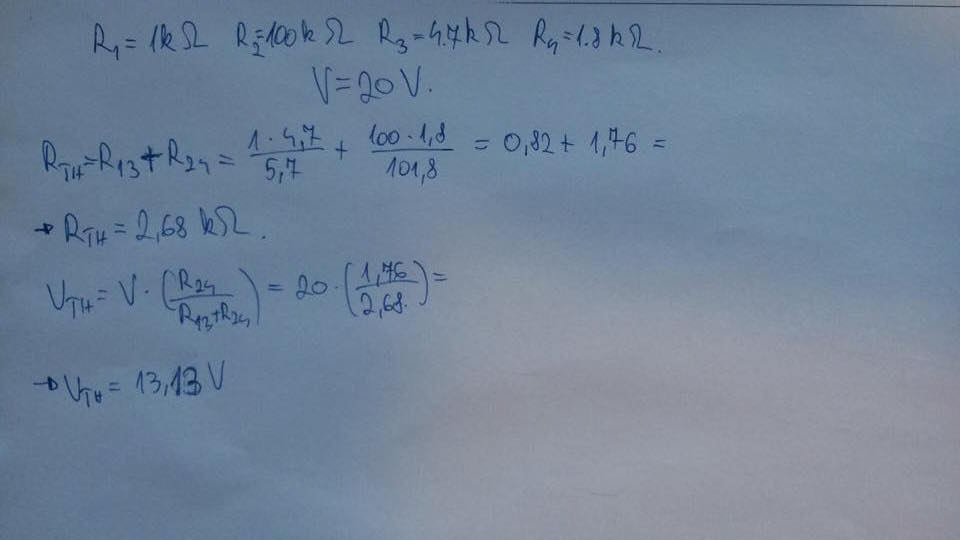
\includegraphics[width=1\textwidth]{images/calc222.jpg}
		\end{figure}
		\newline
		3.After creating the Norton equivalent of the above circuit in the lab, we got the following results:
		
		$V_{TH}=14.25V$, $R_{NO}=2.27k\Omega$, $I_{NO}=6.28mA$
		\newline
		4. We know that $R_{NO}=R_{TH}$ and that $I_{NO}=V_{TH}/R_{TH}$, therefore by taking the values from exercise number 2, we get the following values:
		
		$R_{NO}=2.68k\Omega$ and $I_{NO}=13.13/2.68=4.89mA$
		
	\end{solution}
	\clearpage
	\begin{problem}
		Now we would like to connect a resistor to the output port of the previous circuit.
		\newline
		1. Using the Thevenin equivalent, find the smallest possible resistor for the output port such that the current in the resistor remains less than 1mA.
		\newline
		2. Find and connect the resistance that maximizes the power consumption in the output port.
		\newline
		3. Try several resistors that are higher or lower than your findings, then fill the following table and plot the power curve for a variation of resistors. Compare the results with your calculations.
	\end{problem}
	
	\begin{solution}
		1.After simplifying our circuit using the Thevenin Theorem, we find the a resistor that still satisfies the following criteria:
		
		$V/(R_{TH}+R_{L})<1mA$
		
		So by knowing $R_{TH}$ to be 2.27k$\Omega$, we calculated:
		$x*((2.27*R_{L})/(2.27+R_{L}))= 14.27V$
		
		$1=14.27/2.27+x => x=12k\Omega$	
		
		Answer: 12k$\Omega$ resistor is the smallest possible one for it to remain < 1mA.
		\newline
		2. $R_{L}=R_{TH}=2.27k\Omega$
		\newline
		3.
		\begin{table}[h]
			\begin{tabular}{| l | l | l | l | l | l | l | l | l | l | l | l |}
				\hline
				\textbf{Try} & 1 & 2 & 3 & 4 & 5 & 6 & 7 & 8 & 9 & 10 & 11 \\ \hline
				Resistance (Ohms) & 1.20k & 1.74k & 1.49k & 0.66k & 98 & R\(_{max pow}\) & 2.30k & 2.60k & 2.98k & 5.46k & - \\ \hline
				Voltage (V) & 4.9 & 6.16 & 5.61 & 3 & 0.59 & 0.7 & 7.1 & 7.58 & 8.04 & 10 & - \\ \hline
				Power (mW) & 20 & 21.8 & 21.12 & 13.63 & 3.55 & 0.21 & 21.91 & 22.09 & 21.69 & 18.31 & - \\ \hline
			\end{tabular}
		\end{table}
		
		
		R$_{maxpow}=2.27k\Omega$
		
		$P=V^2/R$
		
		After doing the experiment we realised that $R_{2}$ and $R_{3}$ flipped all along exercise 3.
		
		\begin{figure}[h!]
			\centering
			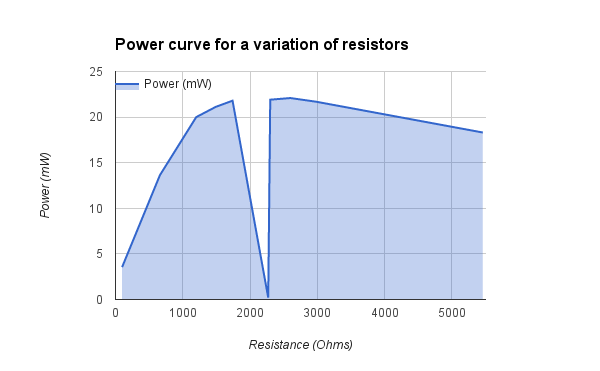
\includegraphics[width=0.8\textwidth]{images/plot233.png}
		\end{figure}
	\end{solution}